%%% TeX代码开始

\documentclass[UTF8,9pt]{ctexbeamer}

\usetheme{Boadilla}

\usecolortheme{beaver}

\usepackage{graphicx}

\usepackage{color}
\usepackage{subfigure}

\setbeamertemplate{caption}[numbered]
\graphicspath{{Images/}}
\begin{document}

\title{{电子元件散热仿真}\\\vspace{1em}}

\subtitle{传热学课程汇报}

\author{\songti {Name}}

\institute{}

\date{\today}

\frame{\titlepage}

\begin{frame}{目录}

\tableofcontents

\end{frame}

\section{物理问题简介}

\begin{frame}{目录}

\tableofcontents[currentsection]

\end{frame}

\begin{frame}

\frametitle{物理问题描述}
%
% \vfill
电子元件安装在PCB板上,使用板状散热器,在自然对流条件下运行。
\\

\begin{figure}
    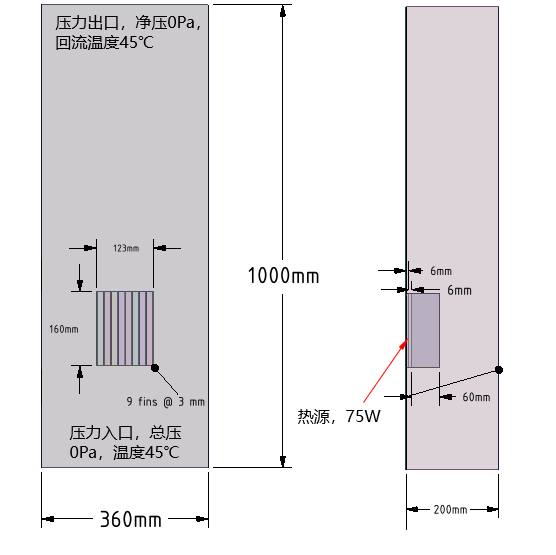
\includegraphics[height=6cm]{figure2.png}
    \caption{问题描述}
\end{figure}
%

%
\end{frame}
\begin{frame}{几何模型}
	注意对各部分共享拓扑。
	\vfill
	\begin{figure}
		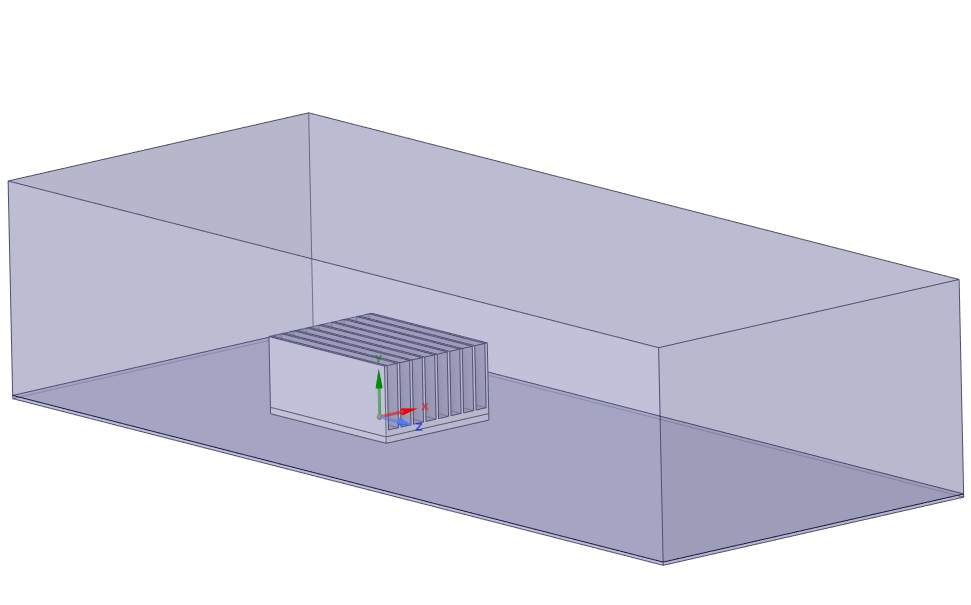
\includegraphics[width=8cm]{figure1.jpg}
		\caption{SCDM中建立的几何模型}
	\end{figure}	
\end{frame}

\section{CFD 仿真过程}

\begin{frame}

\frametitle{目录}

\tableofcontents[currentsection]

\end{frame}


\begin{frame}{网格划分}
	
	\begin{figure}
		\includegraphics[width=8cm, trim={0 5cm 0 1cm}]{060622352924_1.pdf}
		\caption{使用fluent meshing模式划分多面体网格}
	\end{figure}	
\end{frame}
\begin{frame}{模型与方法}
	\begin{table}[]
		\begin{tabular}{l|l}
		\hline
		Model           & Settings           \\ \hline
		Space           & 3D                 \\
		Time            & Steady             \\
		Viscous         & Laminar            \\ 
		Heat   Transfer & Enabled            \\
		Radiation       & Surface to Surface \\
        \hline
		\end{tabular}
		\caption[]{计算模型设置。}
	\end{table}
\end{frame}
\begin{frame}{模型与计算方法}
	\begin{figure}
		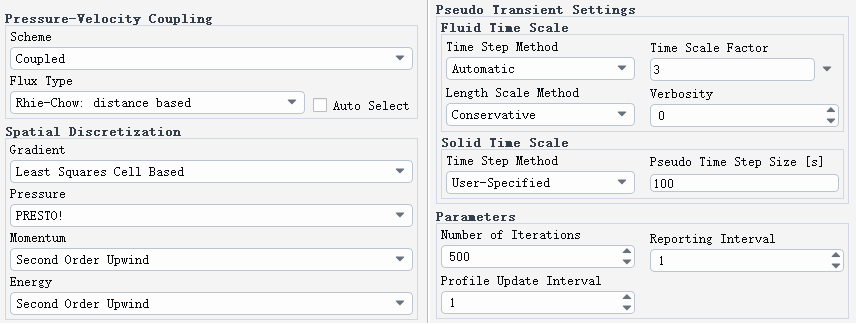
\includegraphics[width=10cm]{figure4.jpg}
		\caption{计算方法}
	\end{figure}	
\end{frame}

\begin{frame}{材料}
	\begin{table}[]
		\begin{tabular}{|cc|}
		\hline
		\multicolumn{2}{|l|}{\textbf{air}}                                        \\ \hline
		\multicolumn{1}{|c|}{Density}              & incompressible ideal gas     \\ \hline
		\multicolumn{1}{|c|}{Cp (Specific Heat)}   & 1006.43 J/(kg K)             \\ \hline
		\multicolumn{1}{|c|}{Thermal Conductivity} & 0.0242 W/(m K)               \\ \hline
		\multicolumn{1}{|c|}{Viscosity}            & 1.7894e-05 kg/(m s)          \\ \hline
		\multicolumn{2}{|l|}{\textbf{component of heat source}}                   \\ \hline
		\multicolumn{1}{|c|}{Density}              & 1900 kg/m\textasciicircum{}3 \\ \hline
		\multicolumn{1}{|c|}{Cp (Specific Heat)}   & 795 J/(kg K)                 \\ \hline
		\multicolumn{1}{|c|}{Thermal Conductivity} & 10 W/(m K)                   \\ \hline
		\multicolumn{2}{|l|}{\textbf{component of PCB}}                           \\ \hline
		\multicolumn{1}{|c|}{Density}              & 1250 kg/m\textasciicircum{}3 \\ \hline
		\multicolumn{1}{|c|}{Cp (Specific Heat)}   & 1300 J/(kg K)                \\ \hline
		\multicolumn{1}{|c|}{Thermal Conductivity} & 0.35 W/(m K)                 \\ \hline
		\multicolumn{2}{|l|}{\textbf{component of heat sink}}                     \\ \hline
		\multicolumn{1}{|c|}{Density}              & 2719 kg/m\textasciicircum{}3 \\ \hline
		\multicolumn{1}{|c|}{Cp (Specific Heat)}   & 871 J/(kg K)                 \\ \hline
		\multicolumn{1}{|c|}{Thermal Conductivity} & 202.4 W/(m K)                \\ \hline
		\end{tabular}
		\caption[]{材料物理特性}
		\end{table}
\end{frame}

\begin{frame}{求解}
	\begin{figure}
		\includegraphics[width=10cm, trim={0 5cm 0 0cm}]{060622352924_3.pdf}
		\caption{迭代过程残差}
	\end{figure}	
\end{frame}
\begin{frame}{求解}
	\begin{table}[]
		\begin{tabular}{|c|c|c|}
		\hline
		\multicolumn{1}{|l|}{}   & Simulation value   & Expected value \\ \hline
		Total heat transfer rate & 74.9808 W          & 75 W           \\ \hline
		Total mass flow rate     & 0.0000007916594 kg & 0              \\ \hline
		continuity residual      & 8.38303E-07        & 0              \\ \hline
		energy residual          & 2.08606E-07        & 0              \\ \hline
		x-velocity residual      & 0.000105974        & 0              \\ \hline
		y-velocity residual      & 0.000195162        & 0              \\ \hline
		z-velocity residual      & 0.000144551        & 0              \\ \hline
		\end{tabular}
		\caption{收敛判据}
		\end{table}	

\end{frame}

\section{仿真结果}

\begin{frame}{目录}
    \tableofcontents[currentsection]
\end{frame}

\begin{frame}{温度}
	\begin{figure}
		\includegraphics[width=10cm, trim={0 4cm 0 1cm}]{060622352924_7.pdf}
		\caption{壁面温度分布}
	\end{figure}
\end{frame}
\begin{frame}{温度}
	\begin{figure}
		\includegraphics[width=8cm, trim={0 3cm 0 1cm}]{060622352924_5.pdf}
		\caption{散热器温度分布}
	\end{figure}	
\end{frame}
\begin{frame}{温度}
	\begin{figure}
		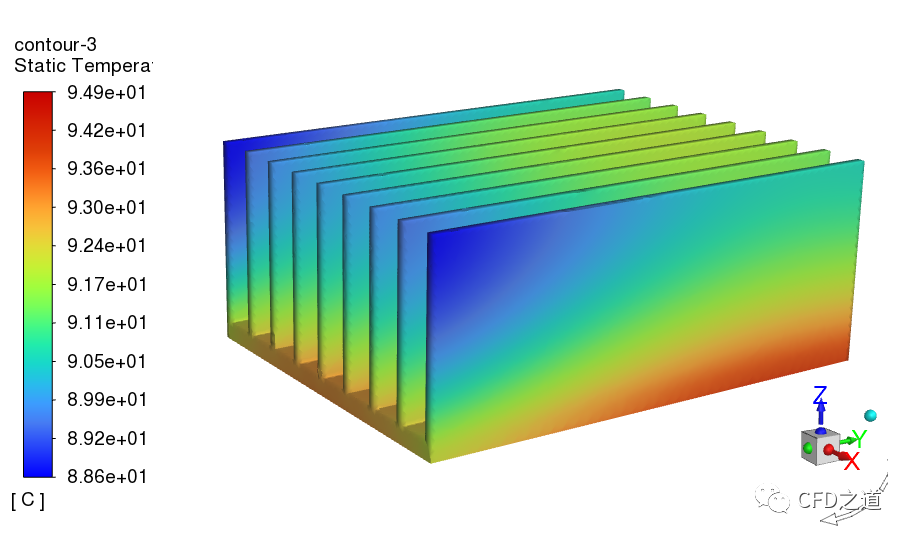
\includegraphics[width=8cm, trim={0 1cm 0 1cm}]{微信图片_20220606231543.png}
		\caption{低速强制对流温度分布(仿真数据)}
	\end{figure}
\end{frame}
\begin{frame}{温度}
	\begin{figure}
		\includegraphics[width=8cm, trim={0 2cm 0 1cm}]{060622352924_6.pdf}
		\caption{散热器底部温度分布}
	\end{figure}
\end{frame}
\begin{frame}{辐射热流密度}
	\begin{figure}
		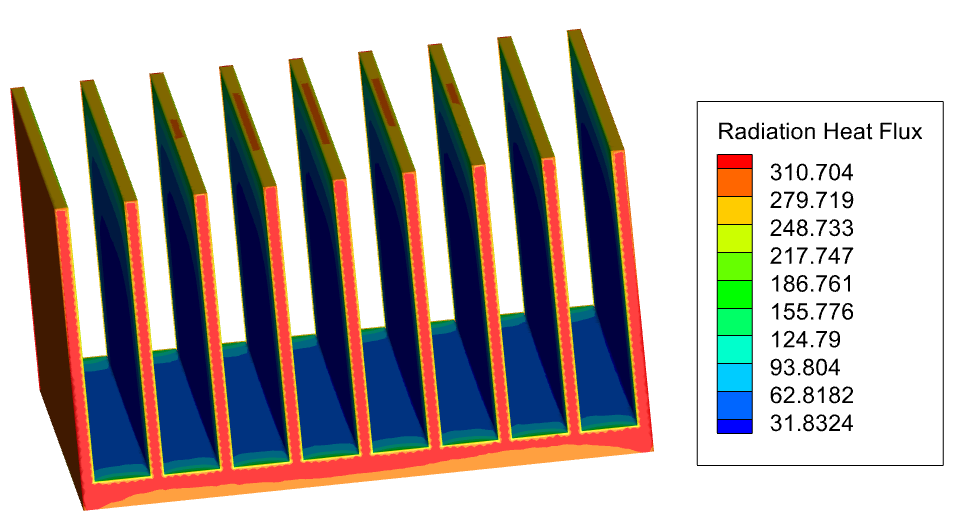
\includegraphics[width=8cm, trim={0 0cm 0 1cm}]{figure15.png}
		\caption{散热器表面辐射热流密度}
	\end{figure}
\end{frame}
\begin{frame}{温度}
	\begin{figure}
		\includegraphics[width=8cm, trim={0 4cm 0 1cm}]{060622352924_8.pdf}
		\caption{散热片中间平面中流体温度分布}
	\end{figure}
\end{frame}
% \begin{frame}{速度}
% 	\begin{figure}
% 		\includegraphics[width=8cm, trim={0 5cm 0 1cm}]{060622352924_10.pdf}
% 		\caption{Contour of Velocity on the center plane of fins.}
% 	\end{figure}	
% \end{frame}
\begin{frame}{速度}
	\begin{figure}
		\includegraphics[width=8cm, trim={0 5cm 0 1cm}]{060622352924_9.pdf}
		\caption{散热片中间平面流线图}
	\end{figure}	
\end{frame}
\begin{frame}{无辐射模型}
	% \vfill
	\begin{figure}[htbp]
		\centering
		\subfigure[]
		{
		%  \begin{minipage}{5cm}
		  \centering
		  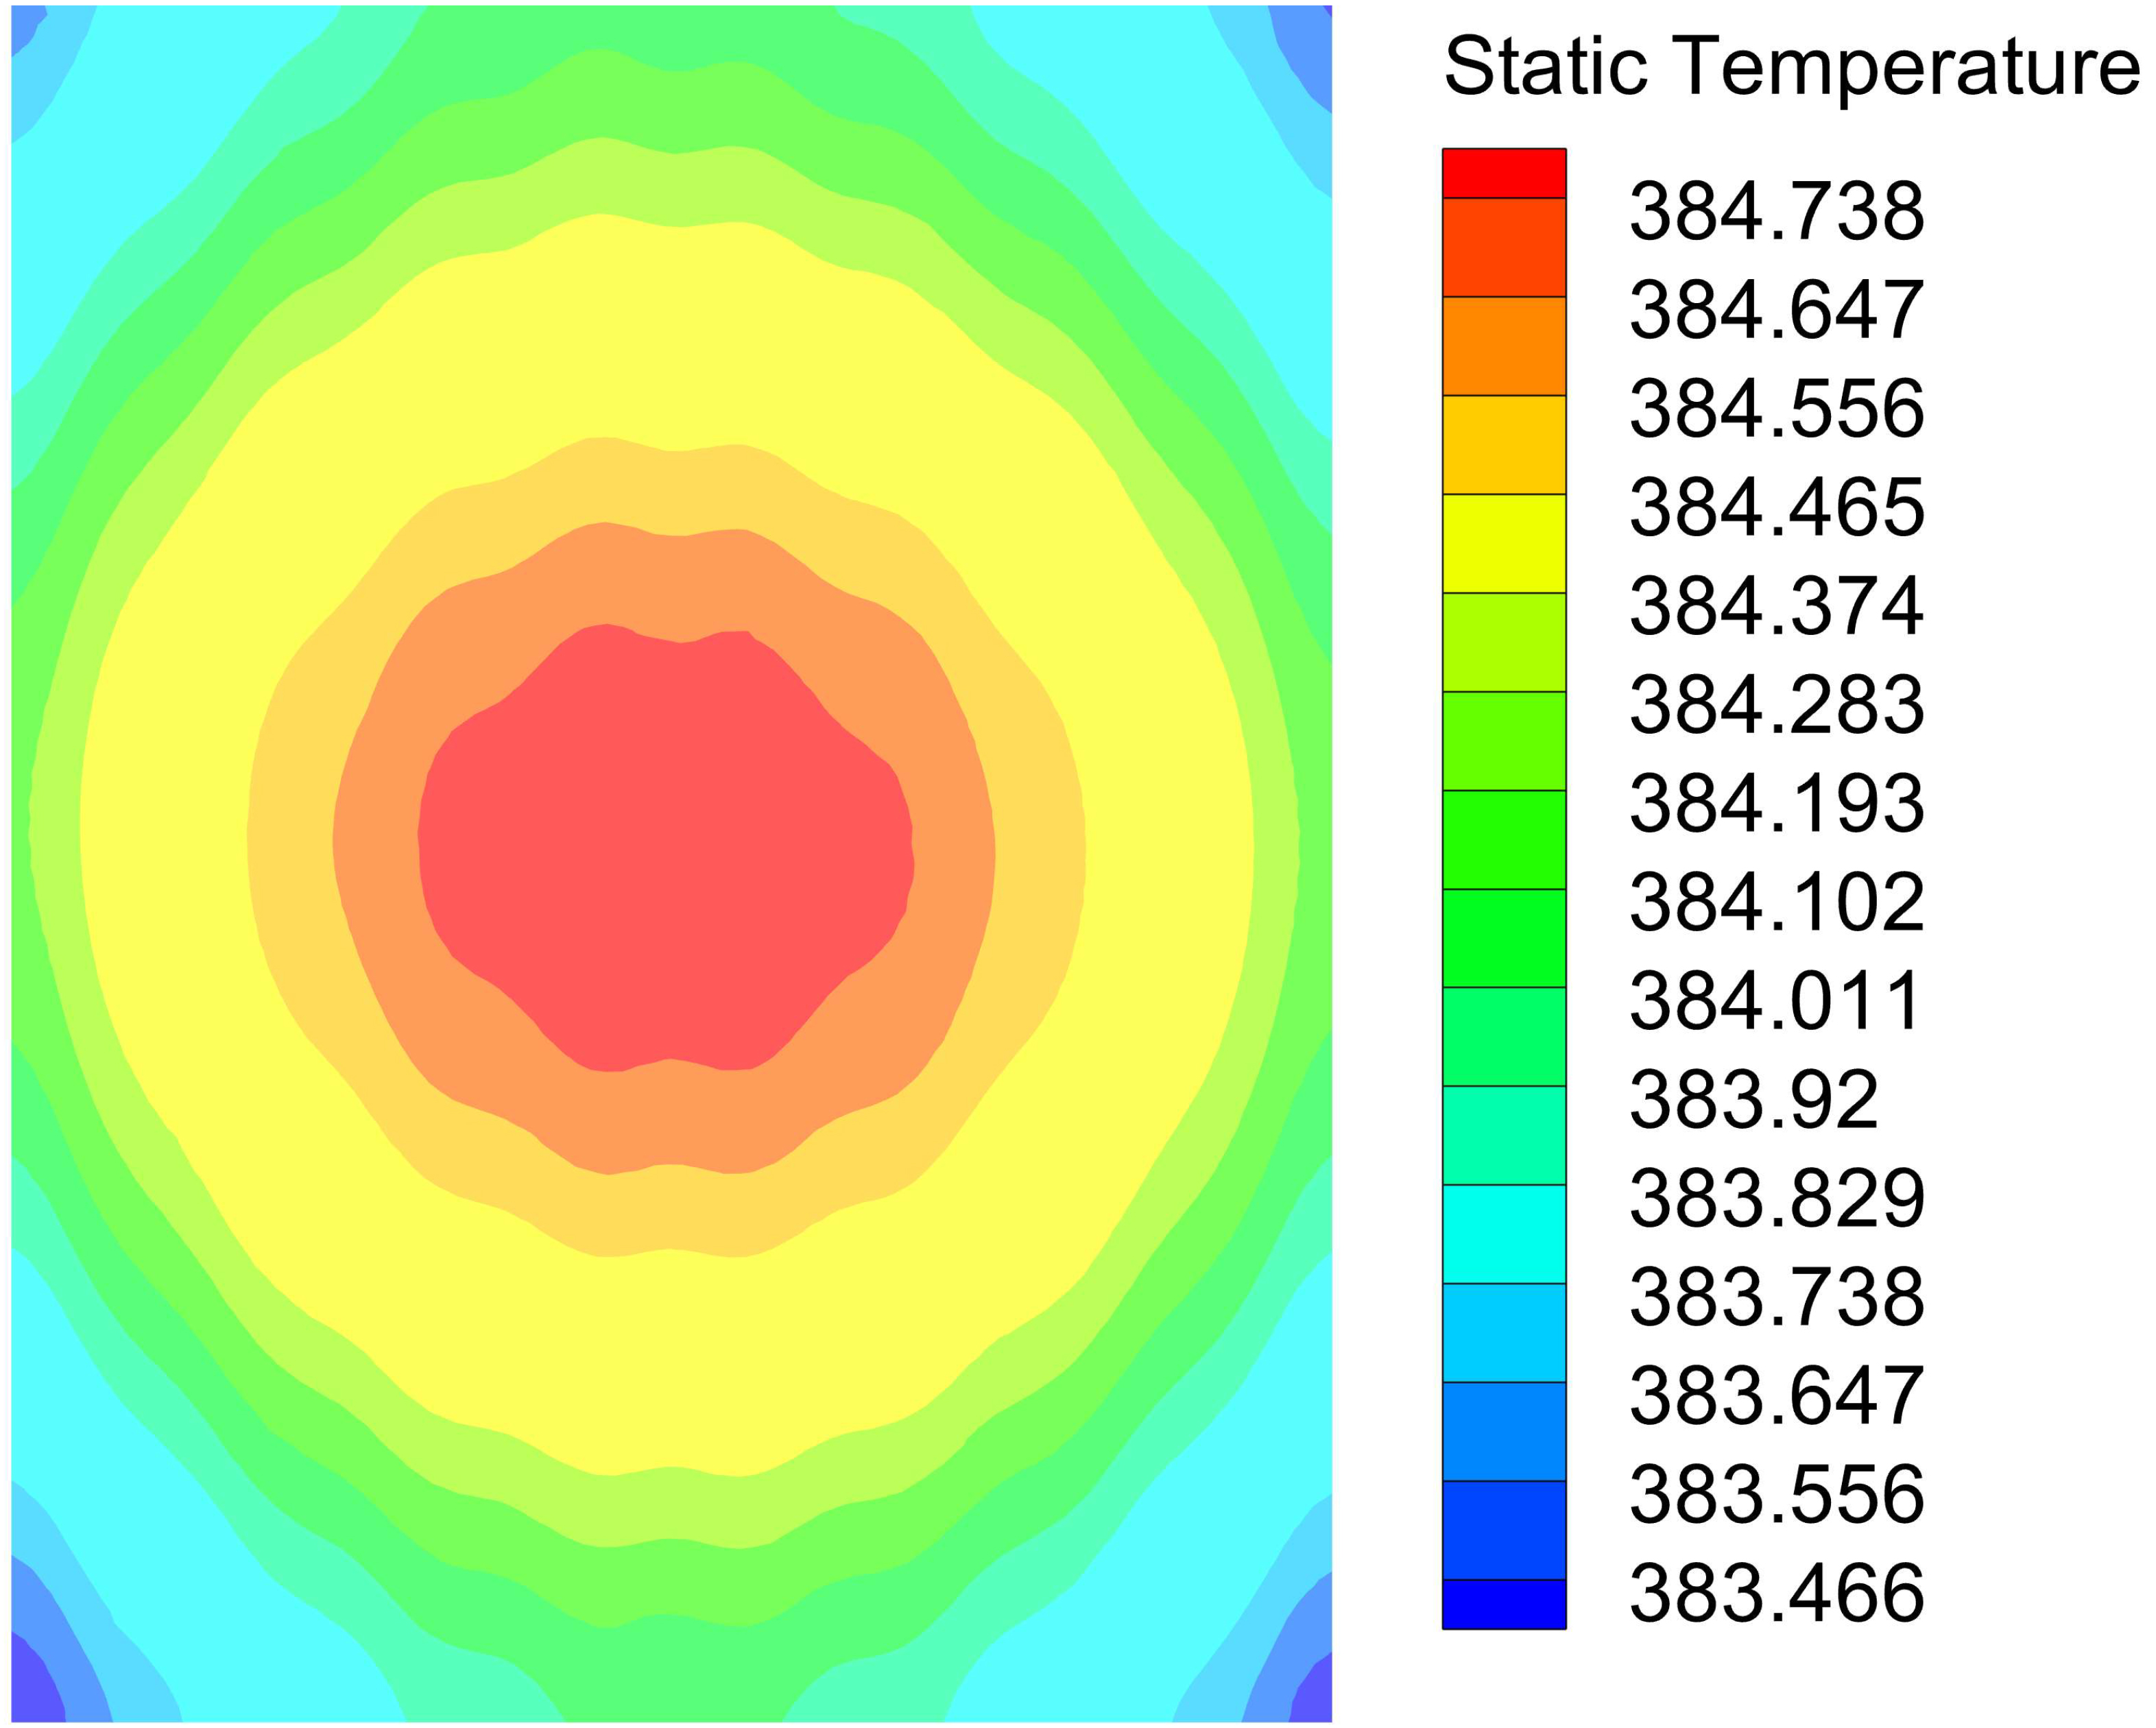
\includegraphics[scale=0.7,width=5cm]{figure14-no.jpg}
		%  \end{minipage}
		}
		   \subfigure[]
		   {
			% \begin{minipage}{5cm}
			 \centering
			 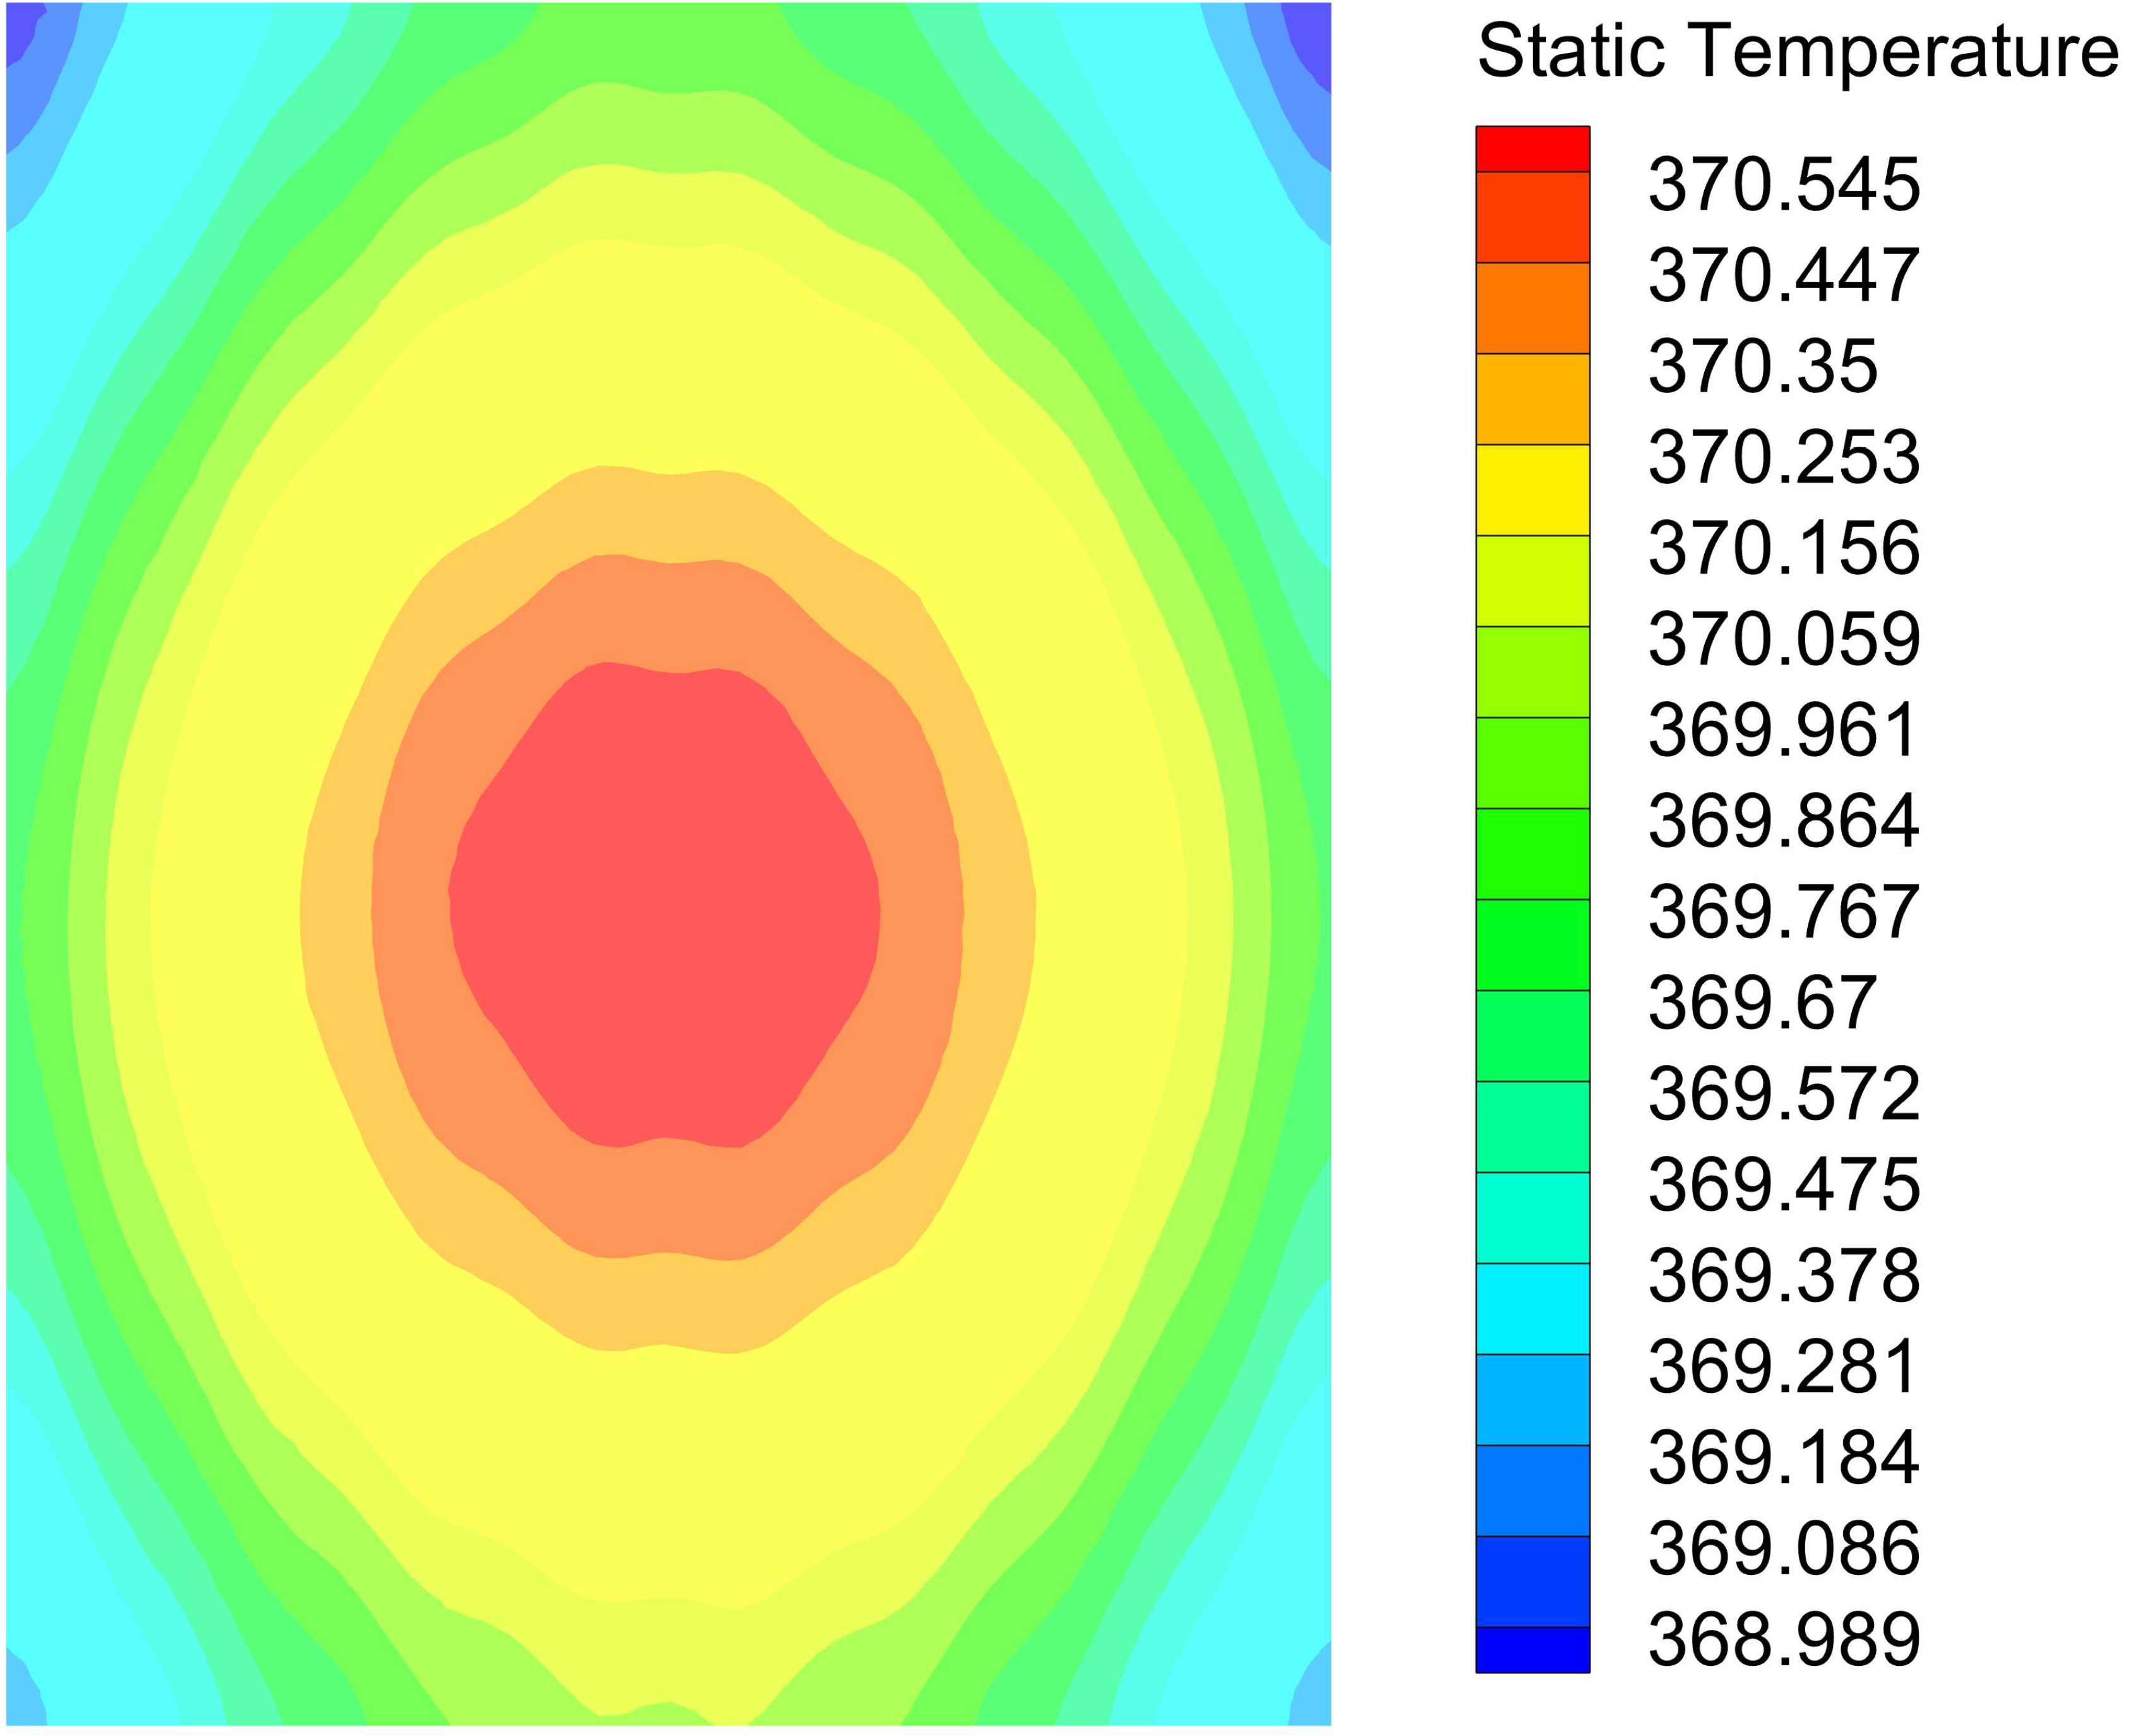
\includegraphics[scale=0.7,width=5cm]{figure14-0.jpg}
			% \end{minipage}
		   }
	   \caption{应用S2S辐射模型前(a)后(b)电子元件表面温度分布}
	   \label{fig:14}
	   \end{figure}
\end{frame}
\end{document}
%%% TeX代码结束
